%------------------------------------------------------------------------------
% $Id: easychair.tex,v 1.23 2008/06/22 17:55:18 mokhov Exp $
%

% Select appropriate paper format in your document class as
% instructed by your conference organizers.
%
% The available formats are 'letterpaper' and 'a4paper' with
% the former being the default if omitted as in the example
% below.
%
\documentclass{easychair}
%\documentclass[a4paper]{easychair}

% In order to save space or manage large tables or figures in a
% landcape-like text, you can use the rotating and pdflscape
% packages. Uncomment the desired from the below.
%
% \usepackage{rotating}
% \usepackage{pdflscape}
%
\usepackage{import}
\usepackage{epstopdf}
\usepackage{bsymb}
\usepackage{alltt}
\usepackage{amsmath}
\usepackage{amssymb}
\usepackage{multicol}
% If you plan on including some algorithm specification, we recommend
% the below package. Read more details on the custom options of the
% package documentation.
%
% \usepackage{algorithm2e}

% Some of our commands for this guide.
%
\newcommand{\easychair}{\sf{easychair}}
\newcommand{\miktex}{MiK{\TeX}}
\newcommand{\texniccenter}{{\TeX}nicCenter}
\newcommand{\makefile}{\texttt{Makefile}}


\makeatletter
\newenvironment{tablehere}
  {\def\@captype{table}}
  {}

\newenvironment{figurehere}
  {\def\@captype{figure}}
  {}
\makeatother


%% Document
%%
\begin{document}

%% Front Matter
%%
% Regular title as in the article class.
%
\title{From Event-B Models to Code}

% \titlerunning{} has to be set to either the main title or its shorter
% version for the running heads. Use {\sf} for highliting your system
% name, application, or a tool.
%
\titlerunning{Event-B Code Generation}

% For only the editors. Authors, please keep this commented out
%\volumeinfo
%	{} % editors
%	{}                         % number of editors
%	{}    % event
%	{}                         % volume
%	{}                         % issue
%	{}                         % starting page number

% Authors are joined by \and and their affiliations are on the
% subsequent lines separated by \\ just like the article class
% allows.
%

\author{Andrew Edmunds\\
School of Electronics and Computer Science,\\
University of Southampton, UK\\
\url{ae2@ecs.soton.ac.uk}\\
\and
Abdolbaghi Rezazadeh\\
School of Electronics and Computer Science,\\
University of Southampton, UK\\
\url{ra3@ecs.soton.ac.uk}\\
\and
Michael Butler\\
School of Electronics and Computer Science,\\
University of Southampton, UK\\
\url{mjb@ecs.soton.ac.uk}\\
\and
Renato Silva\\
School of Electronics and Computer Science,\\
University of Southampton, UK\\
\url{ras07r@ecs.soton.ac.uk}\\
\and
Issam Maamria\\
School of Electronics and Computer Science,\\
University of Southampton, UK\\
\url{im06r@ecs.soton.ac.uk}\\
\and
Chris Lovell\\
School of Electronics and Computer Science,\\
University of Southampton, UK\\
\url{cjl3@ecs.soton.ac.uk}
}

% \authorrunning{} has to be set for the shorter version of the authors' names;
% otherwise a warning will be rendered in the running heads.
%

\authorrunning{Edmunds et al.}

\maketitle

%------------------------------------------------------------------------------
% Abstract
%
\begin{abstract}
Event-B is a formal modelling approach, with good tool support, for use in safety-, and business-critical systems. The methodology supports hierarchical, structured specification, beginning with a high-level abstraction of the system. Detail is added in successive refinement steps, progressing towards implementation. Bridging the abstraction gap, between the modelling and implementation, is addressed in the work that we describe here. Since, at the implementation level, we are concerned with implementation specifics we have chosen to narrow the application domain to that of multi-tasking, embedded control systems. We show how, from an Event-B model, we can generate an abstract model of an implementation, and from this we can generate code. Using an approach that is extensible, we developed back-end code generators for Java, Ada, OpenMP-C and C conforming to the Functional Mock-up Interface for Co-simulation of Cyber-Physical Systems. The extensibility mechanism makes use of the Theory component for translation the mathematical language of Event-B to the target programming language. The approach has been formulated so that it integrates well with the existing Event-B methodology and tools. Event-B is extended with AutoTask, Shared, and Environ machines. We use these features to specify how elements should be translated to code, i.e. controller tasks, protected objects and environment tasks. Using refinement, decomposition, and the extension, we structure projects so that they are amenable to automatic code generation. This necessitates the introduction of a great deal of low-level detail into the specification; so models grow in size considerably. To ensure models remain tractable, we decompose the models (perhaps a number of times). Decomposition encourages modular reasoning, and makes proof more tractable. We make use of an Event-B Composed machine to record the link between the decomposed model. To validate the approach we undertook case-studies, which we use as a running example.
\end{abstract}

\section{Introduction}
Event-B~\cite{ABR10} is one of a number of formal methods that may be used to model systems where a high degree of reliability is required. Event-B was inspired by its predecessor, \emph{Classical-B}~\cite{TheBBook}. It is a modelling language, used with a supporting tool platform, Rodin~\cite{abrial10rodin}; so named from the project in which it was developed~\cite{RodinTool}.  

In this section we introduce Event-B to the reader, and compare Event-B with some other formal approaches. We discuss automatic code generation from formal models, and potential target programming languages.

In Sect.~\ref{} we...
In Sect.~\ref{} we...

\subsection{Event-B}
The formal methods related to the work presented here can be categorized as state-based formal methods. Alternative, but not unrelated, approaches are categorized as process-based methods. Classical-B~\cite{TheBBook,CNP,CNPInterface,B4Free} and its successor, Event-B are said to be state-based, since they focus on modelling the changes of state, not the behaviour of processes. In Classical-B, state updates are modelled by guarded operations, where the operation is an analogue of a procedure call in a programming language. In Event-B, state updates are modelled by guarded events, providing a more abstract view of the way a system evolves. Event-B can be used to model systems at an abstract level; and by adding more detail (using a technique called refinement) it can model the software aspects of systems too. Both methods are set theoretic modelling approaches that incorporate a notion of proof to show that important system properties are maintained. The former is primarily an approach to software systems development, the latter more widely applicable to system-modelling. In an effort to make modelling and proof easier, Event-B was developed to overcome some of the difficulties encountered when using in Classical-B. The main differences between Classical and Event-B are highlighted in~\cite{Hallerstede07}, and inspiration was also drawn from action systems~\cite{Back1990133}.

It is fair to say that Event-B is not just a formal modelling language; the name is used to describe both a notation, and a methodology. In addition to this a mature tool-platform called \emph{Rodin}, named after its development programme, complements the methodology. The main modelling components of Event-B are contexts and machines. Contexts are used to model static features using sets, constants, and axioms. Machines are used to model variable state using \emph{variables}. A third, more recent addition, is the Theory component; where a developer can augment the bundled mathematical language, and rule-base, with new (inference and re-write) rules, data types, and operators. During the modelling process, changes to the components result in automatic generation of proof obligations, which must be discharged in order to show that the development is consistent. The proof obligations generated in classical-B are often complex, the Event-B approach results in simpler proof obligations as described in~\cite{Hallerstede07}, since Event-B consists of a simplified action syntax, giving rise to simpler proof obligations. A further simplification was made by adopting an event-based approach, where each atomic event has a predicate guard and an action consisting only of assignment statements. Events correspond to operations in the B-method; operation specification was more expressive, and included constructs for specifying operation preconditions (as part of its Design by Contract approach), operation calls, return parameters, and more complex structures for branching and looping. These constructs are not features of Event-B. Due to these simplifications (and more efficient proof tools) a large number of the proof obligations may be discharged automatically, by the automatic provers. Where un-discharged proof obligations remain, the user has, at their disposal, an interactive prover. Various techniques can be applied, to discharge the proof obligations, such as adding hypotheses; or making use of the hyperlink-driven user interface, for rule and tactic application. 

As we mentioned earlier in the section, Event-B makes use of a technique called refinement, where a machine can be refined by another. During this process new variables, events and invariant properties can be added; or existing events can be modified, but in a restricted manner. Machine refinement is transitive and leads to a hierarchical structure. Refinements are related to their more abstract counterparts in such a way that, a valid refinement always satisfies the specifications higher in the refinement hierarchy. In this way, important system properties can be specified at a high level of abstraction, and maintained down through the refinement chain. The Event-B tools are responsible for generating the proof obligations relating to refinement; these must be discharged in a similar way to those generated for proof of machine consistency. In some cases we may model entities in an abstraction that are defined in the event parameters; and in the refinement these entities may be introduced to the model as machine variables. To assist with the proof effort, we can link the parameters of the abstract event with their concrete counterpart using a $WITNESS$, this construct is a predicate describing the relationship between the event parameter of the abstraction and a corresponding variable in the refinement. It is often necessary to specify a linking invariant, to describe the relationship between the variables of the abstract and refinement machines. Inspection of the proof obligations can assist in this task since some of the un-discharged proof obligations provide information about this link. Another feature of Event-B is the ability to  refine one atomic event with a number of events, thus breaking the atomicity, as described in~\cite{Butler08}. Eventually, at the end of a refinement chain the models are detailed enough to accurately describe an implementation. But Event-B is a modelling language, and there is a disjunction between the description of the system in Event-B, and commonly used programming languages, such as Java, C and Ada. Addressing the semantic gap between Event-B and programming constructs is the subject of this article, which we will introduce fully, later in the article.

In terms of the recommended methodology, Event-B development begins with the abstraction, and modelling, of the observable events occurring in a system. Event-B (corresponding to its name) takes an event-based view of a system. The event-based approach uses guarded events to describe the observable events. An event is said to be enabled when the guard is true, and the state updates, described in the event actions, can take place; otherwise it is disabled, and none of its updates can occur.  An example of an Event-B machine can be seen in Fig.~\ref{fig:controllerSpec2}. It shows an abstract model of a pump controller, used in one of the case studies. We will use this model to describe some features of Event-B. But first we introduce the case study, which models a discrete \emph{pumpController}. The model describes a system where the controller receives a value of the fluid level, and a boolean value representing a user-request to turn the pump. Based on the inputs to the controller, a command to turn the pump on may be issued, or a warning is issued if a minimum level \emph{MIN} has been reached.    
%
%
%
\begin{figure}
\centering
\begin{minipage}{0.95\textwidth}
\textcolor{blue}{MACHINE} m1 \textcolor{blue}{REFINES} m0 \textcolor{blue}{SEES} ctx \\
\textcolor{blue}{VARIABLES} \text{m\_level, c\_level, e\_level, m\_pumpOnReq, c\_pumpOnReq, e\_pumpOnReq,} \hspace*{0.2cm} m\_pumpOnCmd, c\_pumpOnCmd, e\_pumpOnCmd, m\_warn, c\_warn, e\_warn,\\
\hspace*{0.2cm} c\_level\_internal, c\_pumpOnReq\_internal\\
\textcolor{blue}{INVARIANTS}\\
\hspace*{0.2cm}(c\_level\_internal $\leq$ MIN $\land$  c\_pumpOnReq\_internal = TRUE $\limp$  c\_warn = TRUE)\\
\hspace*{0.2cm} $\land$ (c\_level\_internal $>$  MIN $\land$  c\_pumpOnReq\_internal = TRUE\\
\hspace*{0.5cm} $\limp$  c\_pumpOnCmd = TRUE)\\
\hspace*{0.2cm} $\land$ (c\_level\_internal $\in  \intg$)\\
\hspace*{0.2cm} $\land$ (c\_pumpOnReq\_internal $\in$  BOOL) \ldots\\
\textcolor{blue}{EVENTS}\\
\textcolor{blue}{INITIALISATION} c\_level :=  100 $\pprod$ m\_level := 80 $\pprod$ c\_pumpOnReq :=  FALSE $\pprod$ \ldots\\
\textcolor{blue}{EVENT} fmiSetBoolean\_c \textcolor{blue}{REFINES} fmiSetBoolean\_c\\
\hspace*{0.2cm}\textcolor{blue}{ANY} p\\
\hspace*{0.2cm}\textcolor{blue}{WHERE} p = c\_compound $\land$ p $\in$ BOOL  \\
\hspace*{0.2cm}\textcolor{blue}{THEN} m\_pumpOnCmd :=  p\\
\hspace*{0.2cm}\textcolor{blue}{END}\\
\ldots
\end{minipage}
\caption{An Event-B  Pump Controller Model}
\label{fig:controllerSpec2}
\end{figure}
%
%
%
 In Fig.~\ref{fig:controllerSpec2}, we see that machine \emph{M1} refines another machine, \emph{M0}. It also has a \emph{SEES} clause, to make the contents of a context visible. The context may contain sets, constants, axioms and theorems. There are variables representing the internal state of the controller, and invariants providing type information for variables. Invariants are also used to describe the safety properties of the system. This describes a required safety property, that if the level is at or below \emph{MIN}, and a user's pump-on request is detected, then a warning will be issued. Also, if the level is OK and a pump-on is requested, then the state \emph{pumpOnCmd = TRUE} is  set.  Following the \emph{INVARIANTS} clause are the model's \emph{Events}. The \emph{Initialisation} event is special event, since it has no guards. The initialisation event of a machine must occur before any other event in the machine is enabled. The event in the figure has a parameter \emph{p}, in the \emph{ANY} clause. Parameters can be used to represent information flow, in and out of events, or they can represent a \emph{local} variable within the scope of the event. The event guard is defined in the \emph{WHERE} clause, in the example, where \emph{p} is typed as a Boolean. The guard relates the parameter to a machine variable \emph{c\_pumpOnCmd}, in the predicate $ p = c\_compound$. The event action appears in the \emph{THEN} clause, where the parameter is assigned to the variable \emph{m\_pumpOnCmd}, in the expression $m\_pumpOnCmd := p$.

---




-----
-----

%
%
%
One important aspect of the Event-B approach is that $any$ enabled event may occur, but only one of the enabled events may occur at any one moment. When modelling certain aspects of a system we may wish to impose an ordering of events. However, there is no sequence operator provided in the Event-B approach. It is therefore necessary to make appropriate use of guards and and state variables to model this aspect of a system. For example if we wish to impose an ordering on two events \emph{evt1} and \emph{evt2} so that $evt1$ occurs before $evt2$ we can use the following approach. Introduce an enumerated set $Grds = \{one,~ two,~ stop\}$ and a variable $step~\in~Grds$. Initially $step~\bcmeq~one$; and we make use of $step$ in the event guards as follows,
\begin{equation}
\begin{split}
&evt1 = \textbf{WHEN}~ step = one~ \textbf{THEN}~\ldots\pprod step \bcmeq two~ \textbf{END}\\
&evt2 = \textbf{WHEN}~ step = two~ \textbf{THEN}~\ldots\pprod step \bcmeq stop~ \textbf{END}\\
\end{split}
\notag
\end{equation}
This ensures that initially $evt1$ is enabled and $evt2$ is disabled since $step = one$; only after $evt1$ has updated the $step$ variable  to $two$ is $evt2$ enabled. At this time $evt1$ is no longer enabled since its guard is now false. Finally no events are enabled since $step = stop$ and all guards are false.


\subsection{Related Approaches}



-- VDM


-- Z
\subsection{Code Generation Rationale}


\subsection{Targets for Code Generation}

- Ada

- Java

- FMI-C


\section{An Overview of Event-B}\label{OverviewEB}
The Event-B method~\cite{ ABR10} is a descendant of the classical B-Method~\cite{TheBBook}, and less directly, Z~\cite{Spivey89}. It is a set-theoretic approach to modelling discrete systems, using predicate logic, first order logic, and refinement. The motivation for developing Event-B, from the existing B-Method, was to simplify the task of modelling and proof, and increase the use of automation~\cite{Hallerstede07}. An Event-B development consists of a project containing contexts and machines. Contexts are used to describe the static aspects of a system. Sets and constants are specified, and axioms describe the relationships between them. The dynamic aspects of a system are specified in machines. Machines are able to \emph{see} contexts, so that the contents of a context is visible, and can be used within the machine. Variables keep track of the values, and guarded events update state. The properties of the system are specified in the invariants clause. The invariants of a machine give rise to proof obligations, which are generated automatically by the tool. A large number of these proof obligations can be discharged quickly, by automatic proof tools. Where the automatic provers fail, the user has the opportunity to guide the proof interactively. The proof activity can proceed, with the user suggesting strategies to complete the proof. 
%
\subsection{An Event-B Model}
A fragment of an Event-B specification is shown in Fig.~\ref{fig:TextualEventB}.
%
\begin{figure}
\begin{sffamily}
\begin{minipage}{0.5\linewidth}
%\begin{center}
\begin{tabular}{l}
\textbf{machine} HCtrl\_M1 \\
\textbf{sees} HC\_CONTEXT  \\
\textbf{refines} HCtrl\_M0  \\
\textbf{variables}  cttm cttm2 \ldots \\
\textbf{invariants}\\
\quad  cttm $\in \intg$\\ 
\quad  cttm2 $\in \intg$\\
\qquad  \ldots
\end{tabular}
\end{minipage}
\begin{minipage}{0.5\linewidth}
\begin{tabular}{l}
\quad\textbf{event} Get\_Target\_Temperature2\\
\quad\textbf{any} tm\\
\quad\textbf{where}\\
\qquad  tm $\in \intg$\\ 
\qquad tm = cttm\\
\quad\textbf{then}\\
\qquad cttm2 $\bcmeq$ tm\\
 \quad \textbf{end}
\end{tabular}
\end{minipage}
\end{sffamily}
%\end{center}
	\caption{Example of Textual Event-B}
	\label{fig:TextualEventB}
\end{figure}
%
The specification has a number of variable declarations, which are typed in the \textbf{invariants} clause. Additional predicates are added to the invariants clause to describe the desired safety properties. The machine invariant is a conjunction of the list of predicates in the invariants clause. The \emph{Get\_Target\_Temperature2} event declares one parameter \emph{tm} in the \textbf{any} clause. The \textbf{where} clause contains the event guards, the first clause is a typing predicate for \emph{tm}. The second constrains the value that \emph{tm} can take. The guards describe enabling conditions for an event. Each clause is a predicate over the sets, constants, and variables of the system. All of the guard clauses must be true for an event to be enabled. If an event is enabled, the updates in its action may occur if the event is selected by the environment. Event actions are defined in the \textbf{then} clause; they consist of assignments to machine variables; the assignment may be simple, or non-deterministic. The clause in the example consists of a single, simple assignment, where the variable \emph{cttm2} is assigned the value of the parameter~\emph{tm}.  
\subsection{Machine Decomposition and Event Synchronization}\label{synchDecomp}
Decomposition is a technique that is commonly used to handle complexity. There are currently two styles of composition that can be used with Event-B. They are the shared variable~\cite{AbrialH07}, and shared event~\cite{Butler09a}, styles. In our approach, we make use of shared event decomposition. During the decomposition process, we decide where the machine variables will reside in the decomposed model. In the example of Fig.~\ref{fig:TextualEventB} we put \emph{cttm2} in one machine, and \emph{cttm} in another. Decomposition gives rise to two machines; each with an event called \emph{Get\_Target\_Temperature2}. The event guards and actions will differ though, so it is not just a simple copy. Events can be recomposed following decomposition, to restore the original structure. It can be shown that the recomposed machines refine the original abstract machine, and recomposed events refine their abstract counterparts. The pairs of events, arising from decomposition, are said to synchronize~\cite{Butler2006}. The implementation of synchronized events maps naturally to an atomic subroutine, and we use this in our translation to code.



%------------------------------------------------------------------------------
\section{Tasking Event-B: AutoTask and Shared Machines}\label{TEB}
The Tasking Event-B extension adds a small number of new constructs to Event-B, to facilitate the mapping of Event-B to code. By keeping the number of new constructs to a minimum, and by making use of existing editing tools, we have maintained a small semantic gap between Event-B and the Tasking Event-B specification. The Event-B decomposition approach described in~\cite{Butler09a, decomp2010b} is integral to our methodology. During decomposition, we identify the components of the system, and the interaction between them. We then introduce implementation specific constructs, which the translators use to guide code generation. The extended Event-B model also generates a model of the implementation. 


Tasking Event-B extends Event-B by introducing the concepts of AutoTask, Shared, and Environ Machines. Each machine must be annotated with one of the following, to determine its implementation. AutoTask Machines are related to the concept of an Ada~\cite{ADA2002} task (but we are not restricted to Ada implementations). AutoTask Machines model \emph{controller} tasks in the implementation, and can be viewed as an abstraction of an Ada~\cite{ADA2002} tasks (but we are not restricted to Ada implementations). Shared Machines are related to the concept of a protected resource, such as a monitor ~\cite{Hoare74}, or Ada protected object. Environ Machines model the environment tasks; these will be discussed in the next section. Figure~\ref{fig:route2code} show the development artefacts, and how they relate to the generated code. 
%
\begin{figure}
\centering
		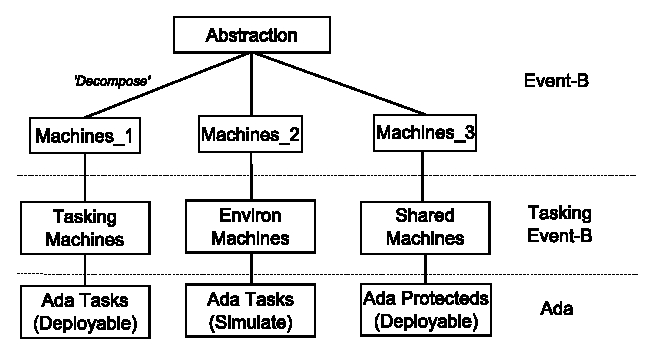
\includegraphics[width=0.7\textwidth]{pictures/route2code.eps}
	\caption{Linking Event-B to Code}
	\label{fig:route2code}
\end{figure}
%

It is possible to generate a simple mapping from Event-B to code, for instance each event can map to a protected procedure. A scheduler can then be used to run the tasks according to a chosen schedule such as~\cite{StoddartCZ07}. We take a different approach, where a task body is used to specify the schedule of activities within a task. We also specify the task life-cycle, such as periodicity of a repeating task, using annotations. These annotations are added to Event-B elements, and are used to guide the translation. The translation of an Event-B machine is characterised by one of the following annotations:
\begin{itemize}
\item  \emph{AutoTask Machine}, \emph{Environ Machine} \emph{Shared Machine}
\end{itemize}
%
AutoTasks are implemented by \emph{controller} tasks, declared and elaborated in the \it Main \rm procedure of the implementation. In Ada, a task declaration is the specification of a task's interface, and an elaboration is the task's implementation. Both parts may reside in the \emph{Main} procedure. All of the tasks, generated from AutoTasks, are created when the program first loads, and automatically activated (made ready to run) by the run-time system; before the \it Main \rm procedure body runs (hence the name AutoTasks). When we compile and build the implementation, we identify the \emph{Main} procedure as the program entry point. In this paper, we only consider AutoTask machines, which are implemented as anonymous tasks of the \emph{Main} procedure. However, in the future we may wish to make use of Ada task types. These are used to create `named' tasks, at compile time; thereby allowing re-use of machine specifications. However, whichever choice we make, fixing the number of tasks, before run-time, is a requirement for compliance with Ravenscar. Therefore, dynamic task allocation is prohibited.
\subsection{Task Scheduling}
The following extensions relate only to AutoTask and Environ machines, and allow a developer to provide implementation details, used by the code generators. Note, however, that timing aspects of periodic tasks, and task scheduling, are not modelled formally in the work that we describe here. 
\begin{itemize}
\item \it TaskType \rm and \it Priority \rm 
\end{itemize}
The \it TaskType \rm construct is used to define the scheduling, cycle and lifetime of a task. i.e. one-shot, periodic or triggered. The period of a task is specified in milliseconds. \it Priority \rm is an integer value; the task with the highest value priority takes precedence when being scheduled. 
\subsection{Flow Control}
The controller tasks of a development are specified using a Tasking Event-B keyword; the machine is annotated with the \emph{AutoTask} keyword. In the generated Ada code, this will be implemented as a controller task, as previously described. Each AutoTask machine has a \emph{task body}.  The task body contains flow control (algorithmic) constructs, which are described in the syntax shown in Fig.~\ref{fig:Syntax}.  The \emph{sequence} construct is used for imposing an order on events. \emph{branch} is choice between a number of events with mutually exclusive guards. \emph{iteration} indicates that an event repeats until its guard is false. \emph{EventSynch} is used to synchronize an event in an AutoTask machine, with an event in a Shared, or Environ machine. The \emph{EventSync} construct defines an atomic update, between AutoTask and Shared machines; synchronization is implemented as an atomic procedure call. Between AutoTask and the Environ machines, synchronization may be implemented as an atomic \emph{entry} call, or by direct access to memory. In Ada, a task \emph{entry} is a kind of subroutine facilitating communication between tasks; it is part of the so-called rendezvous mechanism. It is important to note that, in our approach, controller tasks only communicate with each other through protected objects; however, controller tasks may communicate with environment tasks. 
%
\begin{figure}
\centering
\begin{minipage}{\textwidth}
\begin{tabbing}
TaskBody ::= \\
\quad\= Ta\=skBody ; TaskBody \qquad\qquad \=// sequence\\
\>   $|$ \>\textbf{if} EventSynch \textbf{end} 		\>// branch\\
\>~~[\>\textbf{else if} EventSynch \textbf{end} ] \\
\>~~[\>\textbf{else} EventSynch \textbf{end} ]\\
\>  $|$ \>\textbf{do} EventSynch \textbf{od} \>  // iteration\\
%     [ finally EventSynch ] od	\\
\>  $|$ \>EventSynch	\> // synchronization		\\
\> $|$ \> Output	\>// write to console\\
\\
\\
EventSync ::=			\\
\>\>  Event $\pprod_e$ Event 
\end{tabbing}
\end{minipage}
 \caption{The Task Body Syntax}
 \label{fig:Syntax}
\end{figure}
%
\subsection{Events}
Events can play one of several roles in the mapping to the implementation as follows,
%
\begin{center}
\begin{minipage}{0.9\textwidth}
\begin{tabbing}
\emph{procedureSynch}~  \=- the event is one of a pair of events modelling a parametrized procedure.
\\
\emph{procedureDef}~ \>- the event (on its own) models a non-parametrized procedure.
\\
\emph{branch}~  \>- the event models one part of a branch.
\\
\emph{loop}~  \>- the event models conditional iteration update.
\end{tabbing}
\end{minipage}
\end{center}
%
Events can play one of several roles in the mapping to the implementation. They can take part in event synchronization, parameterless procedure call, part of a branch, part of a loop. The Output construct is provided, to allow developers to output text to a console during simulation. We describe the events of an AutoTask as being \emph{local} with respect to the AutoTask machine, and the events of a Shared machine as being \emph{remote} with respect to the AutoTask machine. Events that are local to an AutoTask machine only update the AutoTask machine state; conversely, events that are remote only update the state of the Shared machine. Synchronised events share parameters to model communication between controller tasks and protected objects, and controller tasks and environment tasks. 
%
An Event-B development typically begins with a high-level abstraction of the system; and we refine, and decompose the models, until we are ready to use Tasking Event-B to describe the implementation. Figure.~\ref{fig:route2code} shows how a development may proceed from abstract model to implementation. The abstract development may be refined, and then decomposed into separate components. In the Tasking Event-B stage, some of the machines are defined as AutoTask Machines; these will be implemented as Ada tasks and used for deployment. Some are defined as Shared Machines; these will be implemented as Ada protected objects and also used for deployment. The remainder are defined as Environ Machines; these will be implemented as the Ada tasks which can be used to simulate the environment. 
%
\subsection{Event Synchronization}
An example of an AutoTask machine with synchronization, and other annotations, is shown in Fig.~\ref{fig:TaskingEventB}.
%
The \emph{EventSync} construct models parameter passing between controller tasks and protected objects. The \emph{EventSynch} construct is represented in concrete syntax by the $\pprod_e$ operator. It can be seen in the figure in a labelled clause in the task body. The label $tc4$ can be translated to a program counter value, as part of the Event-B underlying semantics. This can then be used in invariant clauses to specify properties relating to specific events. In our discussion the labels help to clarify the link between specification and translated code, since we translate them to code comments.

 In Tasking Event-B we match pairs of Event-B parameters in order of declaration, and map them to parameters in procedure declarations or calls. We know that controller tasks call protected objects' procedures, so we determine that  AutoTask events have actual parameters, and Shared machine events have formal parameters. Fig.~\ref{fig:SharedMachine} shows the \emph{SOGet\_Target\_Temperature2} event of the Shared machine, it synchronizes with the \emph{TCGet\_Target\_Temperature2} event of the task shown in Fig.~\ref{fig:TaskingEventB}. 
%

We wish to make a local copy of the Shared machine target temperature $cttm$, in the AutoTask machine,  using the assignment $cttm2 \bcmeq cttm$. However, in preparation for decomposition, we have ensured that the two variables do not appear in a single action; ultimately, \emph{cttm2} and \emph{cttm} will reside in different machines, so the information will need to be passed as a parameter. For this reason we have specified the event as shown in Fig.~\ref{fig:TextualEventB}. There is an action $cttm2 \bcmeq tm$ with guard $tm = cttm$. The decomposition of this event can be seen in Figs.~\ref{fig:TaskingEventB} and~\ref{fig:SharedMachine} with the variables in separate machines.

The event parameters play a role in implementation; they map to the actual and formal parameters in the code. We assist the translator by adding annotations to the parameters, but in theory these could be derived automatically from the machine structure. We retain this as an open issue, for further investigation. During translation, an event's formal parameters will be mapped to formal parameters in a protected object procedure parameter declaration. An event's actual parameters will map to the actual parameters of a call, wherever an \emph{EventSynch} refers to the event in a task body. In Fig.~\ref{fig:TaskingEventB} we see that \emph{tm} is marked as an \emph{actualIn} parameter, and in Fig.~\ref{fig:SharedMachine} \emph{tm} is marked as a \emph{formalOut} parameter. For translation to code, we the match parameters in order of declaration (rather than the names). The \emph{actualIn tm} parameter of the AutoTask event becomes an actual parameter in a call;  and the \emph{formalOut tm} parameter of the Shared machine event becomes a formal parameter in a procedure declaration. The \emph{EventSynch} construct may also be used with just a single event, in which case it is implemented as a procedure call with no parameters. A fragment of the generated code is shown in Fig.~\ref{fig:SynchImpl}. It shows the Ada code from the \emph{SOGet\_Target\_Temperature2} event, and the call to the protected object \emph{s} with the actual parameter \emph{cttm2}. The actual parameter, used in the call, is determined by its appearance on the left-hand-side of the assignment expression in the \emph{TCGet\_Target\_Temperature2} event. 
%
\begin{figure}
\begin{sffamily}
\begin{minipage}{0.5\linewidth}
%\begin{center}
\begin{tabular}{l}
\textbf{machine} Temp\_Ctrl\_TaskImpl \\
\textbf{is autoTask}\\
\textbf{refines} Temp\_Ctrl\_Task\\
\textbf{variables} cttm2, \ldots
\\
\textbf{tasktype} periodic(250) \\
\textbf{priority}  5 \\
\textbf{taskbody is}\\ 
\quad \ldots\\
\quad\textbf{tc4}: TCGet\_Target\_Temperature2 \\
\qquad\quad $\pprod_e$ SOGet\_Target\_Temperature2;   \\
\quad\ldots\\
\end{tabular}
\end{minipage}
\begin{minipage}{0.5\linewidth}
\begin{tabular}{l}
\textbf{event} TCGet\_Target\_Temperature2\\
\textbf{is procedureSynch}\\
\textbf{refines} TCGet\_Target\_Temperature2 \\
\textbf{any}\\
\quad\textbf{actualIn} tm \\
\textbf{where}\\ 
\quad tm $\in \intg$ \\
\textbf{then}\\ 
\quad cttm2 $\bcmeq$ tm \\
\textbf{end}
\end{tabular}
%\end{center}
\end{minipage}
\end{sffamily}
	\caption{Example AutoTask Machine}
	\label{fig:TaskingEventB}
\end{figure}
%
\begin{figure}
\begin{sffamily}
%\begin{center}
\begin{minipage}{0.5\linewidth}
\begin{tabular}{l}
\textbf{machine} SharedObject1Impl\\
\textbf{is sharedMachine} \\
\textbf{refines} SharedObject1 \\
\textbf{variables} cttm \ldots \\
\textbf{invariants} \ldots \\
\end{tabular}
\end{minipage}
\begin{minipage}{0.5\linewidth}
\begin{tabular}{l}
\quad\textbf{event} SOGet\_Target\_Temperature2\\
\quad\textbf{is procedureSynch}\\
\quad \textbf{refines} SOGet\_Target\_Temperature2\\
\quad\textbf{any}\\
\qquad \textbf{formalOut} tm \\
\quad\textbf{where}\\
\qquad tm $\in \intg$\\
\qquad tm = cttm\\
\quad\textbf{then}\\
\qquad skip\\
\quad \textbf{end}\\
\qquad  \ldots
\end{tabular}
\end{minipage}
%\end{center}
\end{sffamily}
	\caption{Example Shared Machine}
	\label{fig:SharedMachine}
\
\end{figure}
%
\begin{figure}
\begin{sffamily}
\begin{minipage}{0.5\linewidth}
\begin{tabular}{l}
s: Shared\_Object1Impl; \\
\ldots \\
\textbf{task body} Temp\_Ctrl\_Task1Impl \textbf{is} \\
\quad \ldots\\
\quad s.SOGet\_Target\_Temperature2(cttm2);\\
\quad\ldots\\
\textbf{end} Temp\_Ctrl\_Task1Impl; 
\end{tabular}
\end{minipage}
\begin{minipage}{0.5\linewidth}
\begin{tabular}{l}
\textbf{protected body} SharedObject1Impl \textbf{is} \\
\quad\textbf{procedure} SOGet\_Target\_Temperature2\\
\qquad\qquad\qquad\qquad\qquad(tm: out Integer) \textbf{is}\\
\quad\textbf{begin}\\
\qquad tm := cttm;\\
\textbf{end};
\end{tabular}
\end{minipage}
\end{sffamily}
	\caption{Ada Implementation of a Synchronization}
	\label{fig:SynchImpl}
\end{figure}
%
\section{Tasking Event-B: AutoTask and Environ Machines}\label{EnvironModel}
The previous section introduced the concept of \emph{AutoTask Machines}~  and \emph{Shared Machines}. We now introduce modelling of the environment, using \emph{Environ Machines}. Controller tasks in the system do not communicate with each other; we prohibit inter-task communication because we wish to support implementations that conform to the Ravenscar profile~\cite{Burns1999, ravenspark}. This profile prohibits the use of the task entries, which are required for inter-task communication. However, we consider that we can relax this restriction, for the \emph{Environ Machines}. This is feasible since the model of the environment will be mapped to simulation code. The remaining deployable code can still be made to conform to the Ravenscar profile, if required. The \emph{Environ Machine}~ is implemented as an Ada task, and communicates with the deployable tasks using Ada's rendezvous mechanism of \emph{entries}. In this paper, we describe the implementations generated from the Environ machine as environment tasks, and the remainder as controller tasks.
%
\begin{figure}
\begin{sffamily}
\begin{minipage}{\linewidth}
\begin{center}
\begin{tabular}{l}
\textbf{event} Sense\_Temperatures \\
\quad\textbf{any} t1 t2 \\
\quad\textbf{where} \\
\qquad t1 $\in \intg$ \\
\qquad t2 $\in \intg$ \\
\qquad t1 = ts1 \\
\qquad t2 = ts2 \\
\quad\textbf{then} \\
\qquad stm1 $\bcmeq$ t1 \\
\qquad stm2 $\bcmeq$ t2 \\
\textbf{end}
\end{tabular}
\end{center}
\end{minipage}
\end{sffamily}
	\caption{An Abstract Sensing Event}
	\label{fig:SensingAbsEvent}
\end{figure}

When modelling embedded control systems it is useful to distinguish between the values we are measuring and setting in the environment, and their internal representation in the controllers. In this paper we describe the values in the environment as monitored or controlled variables (for sensing and actuating respectively). In the controller tasks, the corresponding stored values are described as sensed and actuated variables. 

In a development we use an Environ machine to model the environment. The separation between controller components and environment components is done during decomposition~\ref{synchDecomp}. It is achieved by placing the monitored/controlled variables in one or more machines; and placing the sensed/actuated variables in others. After decomposition, communication between machines is modelled by the synchronization of the events. The implementation of the Environ machine will be somewhat different to that of the Shared machine, seen in the last section. The implementation of the latter uses protected procedures as opposed to task entries. Nevertheless, the annotations are very similar; we now introduce annotations for \emph{sensing} and \emph{actuating} roles. These are added as alternative options to \emph{procedureSynch}, or \emph{procedureDef}, and so on.
%
\begin{center}
\begin{minipage}{0.9\textwidth}
\begin{tabbing}
\emph{sensing}~\quad  \=- the event is one of a pair of events modelling sensing.
\\
\emph{actuating}~ \>- the event is one of a pair modelling actuation.
\\
\end{tabbing}
\end{minipage}
\end{center}
%
The pair of events arising from decomposition (one in the AutoTask machine, the other in the Environ machine) will be annotated to indicate participation in either sensing or actuating roles.

An abstract sensing event can be seen in Fig.~\ref{fig:SensingAbsEvent}. It is the first refinement from the case study presented in Section~\ref{caseStudy}; the model has yet to be decomposed, therefore it has no tasking annotations since these are added as the last step of the development. Sensed variable $stm1$ keeps track of the monitored temperature $ts1$ through the assignment $stm1 \bcmeq t1$, and guard $t1 = ts1$ and so on. Note that the guards $t1 = ts1$ and $t2 = ts2$ link the parameters to the monitored variables. Through decomposition, we obtain the synchronizing events in different machines. 

The \emph{Sense\_Temperatures} event is decomposed into two events, one in each of the machines. In preparation for decomposition we named the AutoTask machine \emph{Temp\_Ctrl\_Task1}, and the Environ machine was named \emph{Envir1}. In a subsequent refinement the events were renamed to \emph{TCSense\_Temperatures} (in the AutoTask machine) and \emph{ENSense\_Temperatures} (in the Environ machine). These events can be seen in Fig.~\ref{fig:SensingEvent}, which show the decomposed events with their Tasking Event-B annotations. The sensed variables \emph{stm1} and \emph{stm2} reside in the AutoTask machine, and can be seen on the left-hand side of the assignment in the \emph{TCSense\_Temperatures} event (on the left side of the figure); and monitored variables \emph{ts1} and \emph{ts2} reside in the in the Environ machine, and appear in the guard of the \emph{ENSense\_Temperatures} event. In Event-B decomposition the order of parameter declaration is not important, synchronization is the same regardless of parameter order. However, in Tasking Event-B we introduce a further constraint on parameter declaration to assist with translation. In translating to code we match parameters in order of declaration. Using this constraint simplifies the translation process; see Sects.~\ref{formalSynch} and~\ref{formalSense} for more details of the mapping from synchronized events to the implementation.
%
\begin{figure}
\begin{sffamily}
\begin{minipage}{0.5\linewidth}
\begin{tabular}{l}
\textbf{event} TCSense\_Temperatures $\triangleq$ \\
\textbf{refines} TCSense\_Temperatures\\
\textbf{sensing} \\
\textbf{begin any} \\
\quad\textbf{actualIn} t1 \\
\quad\textbf{actualIn} t2 \\
\textbf{when} \\
\quad t1 $\in \intg$ \\
\quad t2 $\in \intg$ \\
\textbf{then} \\
\quad stm1 $\bcmeq$ t1 \\
\quad stm2 $\bcmeq$ t2 \\
\textbf{end}
\end{tabular}
\end{minipage}
\begin{minipage}{0.5\linewidth}
\begin{tabular}{l}
\textbf{event} ENSense\_Temperatures $\triangleq$ \\
\textbf{refines} ENSense\_Temperatures \\
\textbf{sensing} \\
\textbf{begin any} \\
\quad\textbf{formalOut} t1 \\
\quad\textbf{formalOut} t2 \\
\textbf{when} \\
\quad t1 $\in \intg$ \\
\quad t2 $\in \intg$ \\
\quad t1 = ts1 \\
\quad t2 = ts2 \\
\textbf{then} \\
\quad skip \\
\textbf{end}
\end{tabular}
\end{minipage}
\end{sffamily}
	\caption{Synchronization of a Sensing Event}
	\label{fig:SensingEvent}
\end{figure}
%
\section{Case Study}\label{caseStudy}
This section describes an Event-B development of a simple heating controller. This case study covers the entire development process; starting from a system specification and ending with implementable Ada code. The methodology that we propose here is key to optimising the development process, since the abstract development must be structured in a way that is appropriate for code generation. The development process starts with an abstract specification followed by two successive refinements. We then decompose the model into two separate sub-models, one representing the environment, and the other representing the remainder of the system. The refinement process continues after the first decomposition in order to arrive at a concrete level suitable for implementation. This allows us to derive the appropriate machine structure, needed by the code generation plug-in. The second decomposition gives rise to a number of AutoTask machines, and a Shared machine to manage the protected shared data. The Shared machine synchronizes with the AutoTask machines to model the communication between them. We illustrate how, using the code generation plug-in, a concurrent Ada implementation is generated. The overall aim of this case study is to put in practice the recommended methodological aspects of Event-B, particularly those aspects of modelling concerned with decomposition and code generation.
\subsection{Overview of the System}
%
\begin{figure}
	\centering
		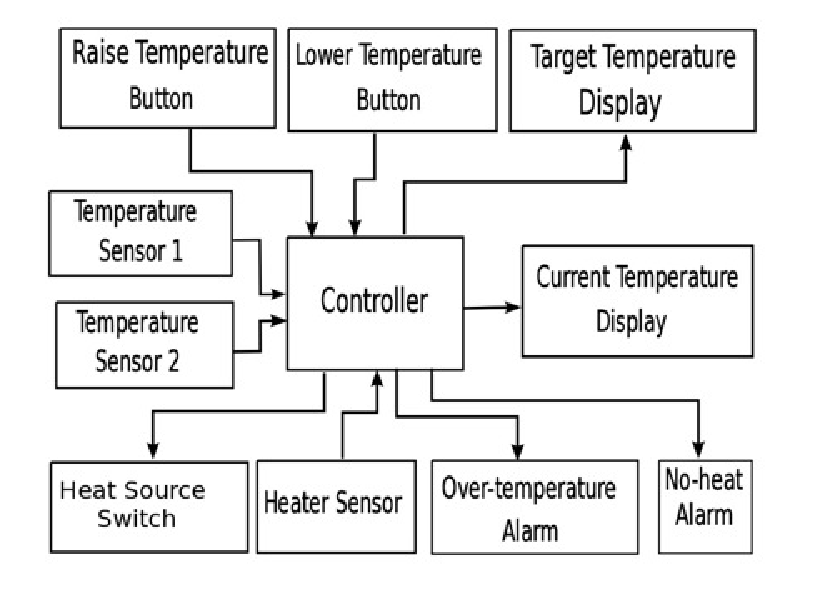
\includegraphics[width=0.5\textwidth]{pictures/arch.eps}
	\caption{Heating Controller Architecture}
	\label{fig:arch}
\end{figure}
Figure~\ref{fig:arch} shows an overview of the Heating Controller and related components. The controller in the centre of the diagram communicates with the components in the environment using input and output parameters. At the top there are two buttons that allow the user to increase/decrease Target Temperature. The target temperature periodically will be sent by the controller to the related display to be shown to the outside world. The controller uses two Temperature Sensors to poll the environment temperature. The average of the values read from these two sensors is calculated and displayed by the controller on the Current Temperature Display. If the current temperature is lower than the target temperature, the controller will turn on the heater source using Heat Source Switch, otherwise this switch will be turned off by the controller. The status of the heater itself also will be monitored through the Heater Sensor. If due to some faults the heater is not working properly, the controller will activate either of Over-temperature Alarm or No-heat Alarm.  
%
\subsection{System Development}
%
Before discussing Event-B models the Heater Controller in more detail, we provide an overview of the development approach in Fig.~\ref{fig:devel}.
%
\begin{figure}
	\centering
		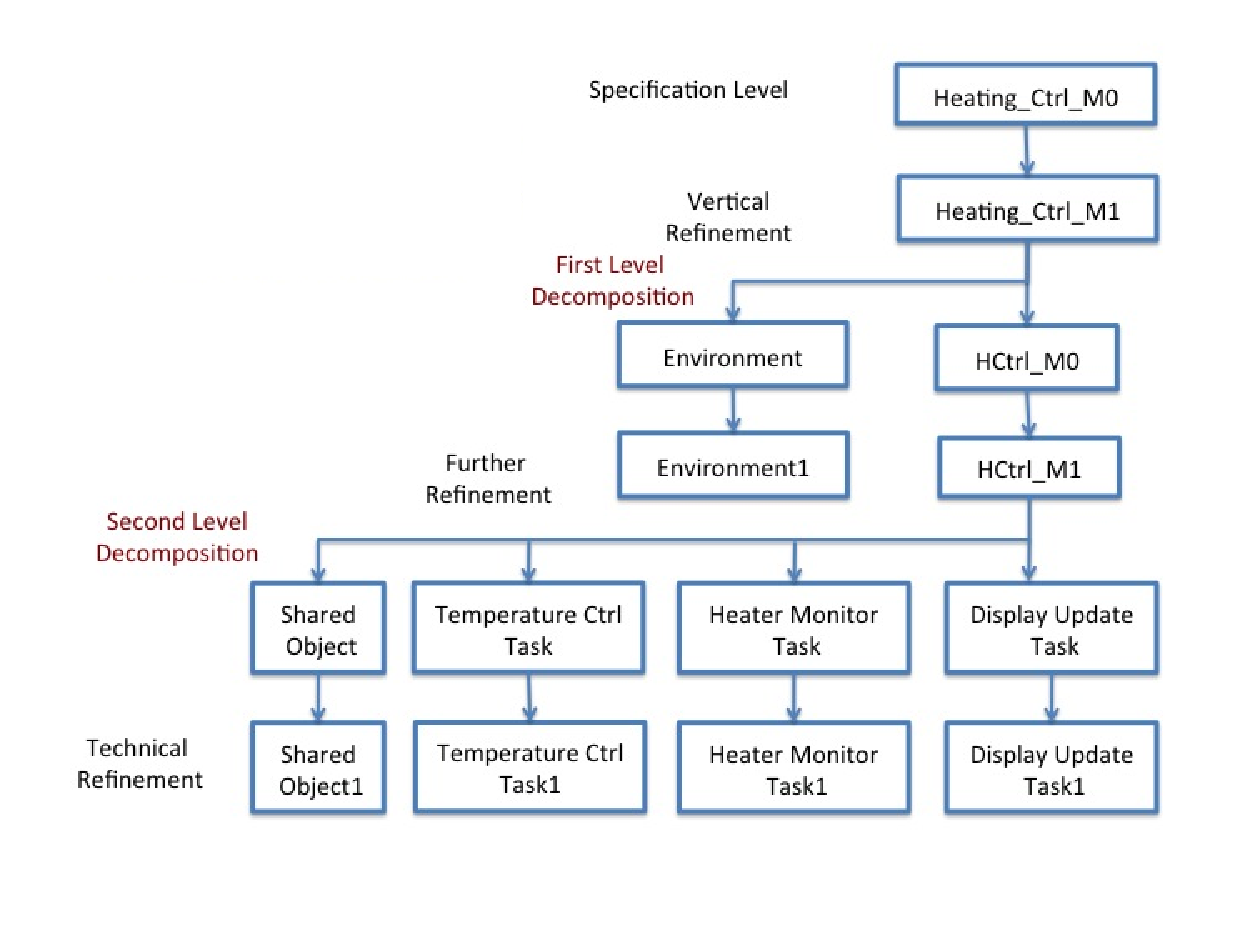
\includegraphics[width=0.7\textwidth]{pictures/devel.eps}
	\caption{The Development Approach}
	\label{fig:devel}
\end{figure}
%
Starting from the top level of the diagram, it shows the most abstract model of the system, or as it is known - the system specification. At the top level we specify the system's main functionality. This includes events for modelling increase/decrease target temperature, polling the environment temperature using the two available sensors, calculating the current temperature, turning on/off the heat source, and activating/deactivating the two different alarms. Events at this level are deliberately simple, to keep the specification clear and concise. Event ordering and iteration are introduced in the later stages. In the first refinement we introduce sensing and actuation, which are considered to be design steps. Sensing events model the polling of the state of the increase/decrease buttons, the temperature sensors, and the heater sensor. Actuating events model the updates of target, and current temperature displays. The also model actuation occurring as a result of controller decisions, such as turning the heat on/off, and activating the various alarms. 

As illustrated in Fig.~\ref{fig:devel} we decompose our model in two stages. In the first stage we separate the controller, the part of the system that should be implemented, from its surrounding environment. The second stage of decomposition is concerned with the tasking structure of the implementable system. The structure of a particular development is determined by the developer, based on their understanding of the required implementation.
%
\subsubsection{First Decomposition}
%
In Event-B, we usually start modelling by specifying the whole system as a closed system. This includes the system that we are intending to develop and its surrounding environment. Therefore when our model of the system becomes large and complex it is reasonable to separate the controller from its environment. Hence in the first stage of decomposition, we partition our model into those two parts, as shown in Fig.~\ref{fig:decomp1}. The environment machine models all of the external parts of the system that the controller interacts with. These include buttons, sensors, actuators and their related behaviours. In addition to modelling updates in the components, the machines modelling the environment and controller, also model the synchronisation between the two.
%
\begin{multicols}{2}
\begin{figurehere}
	\centering
		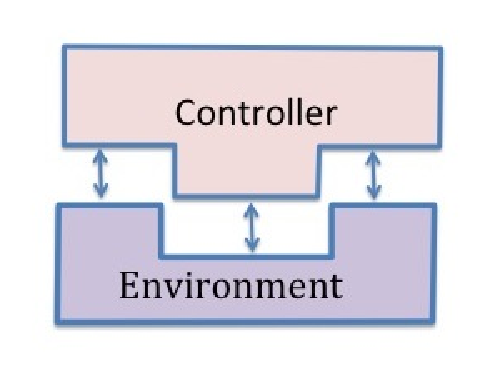
\includegraphics[width=0.4\textwidth]{pictures/decomp1.eps}
	\caption{Decomposition - Stage 1}
	\label{fig:decomp1}
\end{figurehere}

\begin{figurehere}
	\centering
		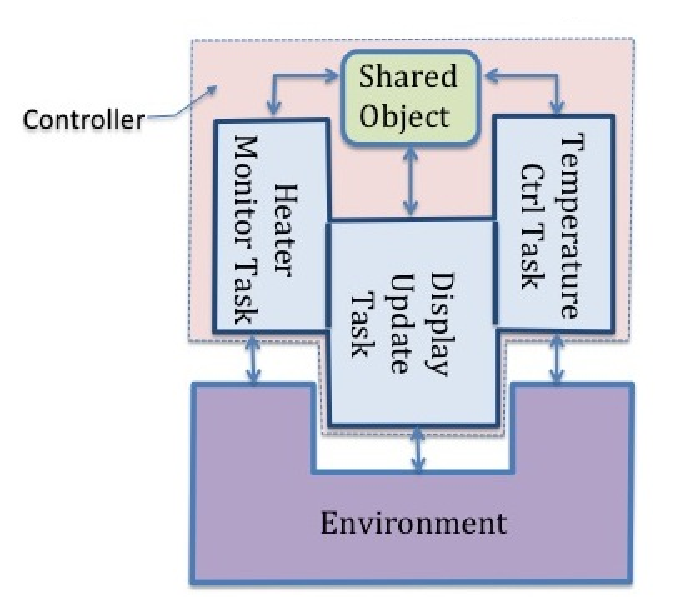
\includegraphics[width=0.4\textwidth]{pictures/decomp2.eps}
	\caption{Decomposition - Stage 2}
	\label{fig:decomp2}
\end{figurehere}
\end{multicols}
%
\subsubsection{Second Decomposition}
%
In this, the second stage of decomposition, we decompose the controller into three different tasks which interact with each other through a protected object. This structure is presented in Fig.~\ref{fig:decomp2}.
%
Note that individual tasks are able to communicate with the environment directly, but do not communicate with each other. In practice, the number of tasks, and the way that we distribute different events over these tasks is determined by various factors. Other properties of tasks, such as their priorities; life-cycle (periodic, triggered etc); length of period in milliseconds, if applicable, are defined later using Tasking Event-B.
%
\subsection{Tasking Event-B}
When we are ready to start adding implementation level details to the model we use Tasking Event-B annotations; entering the \emph{Tasking Event-B} modelling stage shown in Fig.~\ref{fig:route2code}. We do not present the whole case study specification here, but we use extracts to illustrate the main issues. In the following discussion we use the temperature control task event \emph{Temp\_Ctrl\_Task1Impl} from Fig.~\ref{fig:TaskingEventB}, as an example. Our main aim is to highlight how we use Tasking Event-B to facilitate the task's interaction with the environment, but we also discuss the task's behaviour in a more general sense. The first step is to use annotations to identify the machines, as one of AutoTask, Environ or Shared machines. When we have identified machines as either Environ, or AutoTask, then we add a task body specification. The task body is used to constrain the Event-B model, in such a way that it can be implemented using commonly available programming constructs, such as sequence, branch and subroutine calls. The generated code can be viewed as an implementation of a schedule of events. Fig.~\ref{fig:taskBody} shows the \emph{Temp\_Ctrl\_Task1Impl} task body. The clauses of the task body are labelled, to assist with translation, and the following list describes the behaviour of the events  that they refer to.
%
\begin{figure}[h]
\centering
\begin{minipage}{\textwidth}
\begin{tabbing}
tc1 - \=a sensing synchronization that models polling of the $ts1$ and $ts2$  temperature sensors,\\
 \>as shown in Fig.~\ref{fig:SensingEvent}. \\
tc2 - \>an update that calculates, and stores locally, the average of the two temperature values. \\
tc3 - \>an actuating synchronization that updates $ctd$, the displayed temperature. \\
tc4 - \>a procedure synchronization that gets the target temperature from the protected object. \\
tc5 - \>branching choice: set the heater on or off flag in the task. \\
tc6 - \>a procedure synchronization that sets the heat source active flag in the protected object. \\
tc7 - \>an actuating synchronization that updates $ahsa$, the activate heat source flag. \\
tc8 - \>a branching choice: set activate overheat alarm flag in the task. \\
tc9 - \>an actuating synchronization that updates $aota$, the activate overheat alarm flag. 
\end{tabbing}
\end{minipage}
\end{figure}
%
\begin{figure}
\begin{sffamily}
\begin{center}
\begin{minipage}{0.8\linewidth}
\begin{tabular}{l}
tc1: TCSense\_Temperatures $\pprod_e$ ENSense\_Temperatures; \\
tc2: TCCalculate\_Average\_Temperature; \\
tc3: TCDisplay\_Current\_Temperature $\pprod_e$ ENDisplay\_Current\_Temperature; \\
tc4: TCGet\_Target\_Temperature2 $\pprod_e$ SOGet\_Target\_Temperature2; \\
tc5: \textbf{if} TCTurnON\_Heat\_Source \textbf{end if} \\
\qquad \textbf{else} TCTurnOFF\_Heat\_Source \textbf{end else}; \\
tc6: TCSet\_Heat\_Source\_State $\pprod_e$ SOSet\_Heat\_Source\_State; \\
tc7: TCActuate\_Heat\_Source $\pprod_e$ ENActuate\_Heat\_Source; \\
tc8: \textbf{if} TCSwitchOn\_OverHeat\_Alarm \textbf{end if} \\
\qquad \textbf{else} TCSwitchOff\_OverHeat\_Alarm \textbf{end else}; \\
tc9: TCActuate\_OverHeat\_Alarm $\pprod_e$ ENActuate\_OverHeat\_Alarm 
\end{tabular}
\end{minipage}
\end{center}
\end{sffamily}
	\caption{The Temp\_Ctrl\_Task1Impl Task Body}
	\label{fig:taskBody}
\end{figure}
%
The task body gives rise to the Ada task body of Fig.~\ref{fig:tempTask}. 
%
\begin{figure}
\begin{sffamily}
\begin{center}
\begin{minipage}{\linewidth}
%\begin{tabular}{l}
\begin{tabbing}
\textbf{task body} Temp\_Ctrl\_Task1Impl \textbf{is} \qquad\qquad\qquad\qquad\qquad\qquad\qquad \= \\
\quad$\ldots$  \\
\quad\textbf{procedure} TCCalculate\_Average\_Temperature \textbf{is} \\
\quad\textbf{begin} \\
\qquad avt := ((stm1 + stm2) / 2); \\
\quad\textbf{end}; \\
\quad\textbf{begin} \\
\quad$\ldots$ \\
\quad   Envir1Impl.ENSense\_Temperatures(stm1, stm2); \>$--~tc1$\\
\quad    TCCalculate\_Average\_Temperature; \>$--~tc2$ \\
\quad    Envir1Impl.ENDisplay\_Current\_Temperature(avt); \>$--~tc3$ \\
\quad    shared\_object1implInst.SOGet\_Target\_Temperature2(cttm2); \>$--~tc4$ \\
\quad    \textbf{if}(avt $<$ cttm2) \textbf{then} \>$--~tc5$ \\
\qquad        hsc := TRUE;\\
\quad    \textbf{else} \\
\qquad        hsc := FALSE; \\
\quad    \textbf{end if}; \\
\quad    shared\_object1implInst.SOSet\_Heat\_Source\_State(hsc); \>$--~tc6$  \\
\quad    Envir1Impl.ENActuate\_Heat\_Source(hsc); \>$--~tc7$\\
\quad    \textbf{if}(avt $>$ Max) \textbf{then} \>$--~tc8$ \\
\qquad        ota := TRUE; \\
\quad   \textbf{else} \\
\qquad        ota := FALSE; \\
\quad    \textbf{end if}; \\
\quad    Envir1Impl.ENActuate\_OverHeat\_Alarm(ota); \>$--~tc9$ \\
\quad$\ldots$ \\
\textbf{end} Temp\_Ctrl\_Task1Impl; 
\end{tabbing}
%\end{tabular}
\end{minipage}
\end{center}
\end{sffamily}
	\caption{Implementation of Temp\_Ctrl\_Task1Impl Task Body}
	\label{fig:tempTask}
\end{figure}

The development proceeds by adding annotations to events; we saw annotated sensing events in Fig.~\ref{fig:SensingEvent}. The $sensing$ keyword is used with the $TCSense\_Temperatures$ and $ENSense\_Temperatures$ events. This indicates that the events model polling of the environment; the $actuating$ keyword is similar, except that it indicates that events update values is the environment. The clause $tc1$ in the task body, shown in Fig.~\ref{fig:taskBody}, gives rise to the following Ada program statement:
\\\\
\begin{minipage}{\textwidth}
\begin{center}
\begin{sffamily}
Envir1Impl.ENSense\_Temperatures(stm1, stm2); $\qquad--tc1$
\end{sffamily}
\end{center}
\end{minipage}
\\\\
\emph{Envir1Impl} is the name of the environment task, and \emph{ENSense\_Temperatures} is the name of the task entry. The sensed variables $stm1$ and $stm2$, appear in the actions of $TCSense\_Temperatures$. The action models assignment of return values to the variables. In the translation to Ada the AutoTask event parameters is replaced by machine variables, and the variables are passed as actual parameters in an entry call. The entry is implemented as an Ada $accept$ statement, see Fig.~\ref{fig:senseTempImpl}, in the $Envir1Impl$. In the body, statements assign the temperature values $ts1$ and $ts2$ to the formal parameters $t1$ and $t2$. The variables $ts1$ and $ts2$ were added to the Event-B model, in a refinement step, to represent the monitored values in the environment. The monitored variables appear in the guard of the $ENSense\_Temperatures$ event. See Fig:~\ref{fig:SensingEvent}. With Ada's pass-by-result parameter semantics, the assignment statement $t1 \bcmeq ts1$ ensures $stm1$ is assigned the value of $ts1$ upon return. More details of the translation of synchronized events can be found in Section~\ref{formalSynch}.
%
\begin{figure}
\begin{sffamily}
\begin{minipage}{\linewidth}
\begin{center}
\begin{tabular}{l}
\textbf{accept} ENSense\_Temperatures(t1: \textbf{out} Integer; t2: \textbf{out} Integer) \textbf{do} \\
\quad t1 $\bcmeq$ ts1; \\
\quad t2 $\bcmeq$ ts2;\\
\textbf{end} ENSense\_Temperatures;
\end{tabular}
\end{center}
\end{minipage}
\end{sffamily}
	\caption{Implementation of ENSense\_Temperatures}
	\label{fig:senseTempImpl}
\end{figure}
%
\section{Writing Directly to Memory Locations}\label{direct}
The discussion, so far, has focussed on a simulation of the environment whereby the task communicates with the environment using an entry call. In Ada this is implemented as an entry call to the environment task. It may be the case, however, that the developer can specify some memory locations to read from, and write to, directly. Our approach allows developers to annotate event parameters with the address information. We have introduced the $addr$ annotation, with which we define an addressed variable. It is used in conjunction with the existing $actualIn$. $actualOut$, $formalIn$, and $formalOut$ annotations. With $addr$ we can specify  a memory location and its number base. In the Tasking Event-B specification, on the left of Fig.~\ref{fig:AddressedVars}, the parameter $t1$ is given the address $ef14$ in base 16. We can see, on the right, the generated Ada code. The parameter $t1$ has been mapped to the integer variable declaration \sffamily t1:~Integer\rmfamily. The address of the variable has been set using the following statement, the \textbf{pragma} Atomic(t1) statement is used to indicate that any access to $t1$ must occur atomically:
\begin{center}
\begin{minipage}{\textwidth}
\begin{tabbing}
\=\textbf{for} t1'Address \textbf{use} System'To\_Address(16\#ef14\#);\\
\>\textbf{pragma} Atomic(t1);
\end{tabbing}
\end{minipage}
\end{center}
%
In Ada this is known as an $address~clause$. In the Ada $TCSense\_Temperatures$ procedure, also shown in Fig.~\ref{fig:AddressedVars}, the variable $t1$ appears on the right-hand side of the assignment. When the statement is executed, the value is read from the memory location accessed by $t1$, and assigned to $stm1$. If we were generating C code, we would declare a pointer to integer type,
\begin{center}
\begin{minipage}{0.22\textwidth}
\textbf{int}* t1 = (\textbf{int}*) 0xef14
\end{minipage}
\end{center}
and use an assignment  stm1 = *t1 . We can see that this approach differs from that of the entry-call approach shown earlier; the controller task updates its value without a call to an external, environment entry. Now, since there is no call to an entry (which is atomic) the environment must be responsible for ensuring that sensing events with multiple read actions, and actuating events with multiple write actions, are performed atomically. When using addressed variables, in Tasking Event-B, we can discard the environment tasks, and simply use the controller tasks and protected objects in the deployment. In this case we need not consider the effects of atomicity further. However, we may wish to use the environment model for other purposes,  in which case we need to ensure that atomic access is achieved in the code.
%
\begin{figure}[b]
\begin{sffamily}
\begin{minipage}{0.45\linewidth}
\begin{center}
\begin{tabular}{l}
\textbf{event} TCSense\_Temperatures $\triangleq$ \\  
\textbf{refines} TCSense\_Temperatures \\
\textbf{sensing} \\
\textbf{begin any} \\ 
\quad \textbf{actualIn}~~\textbf{addr}(16,ef14) t1 \\
\quad \textbf{actualIn}~~\textbf{addr}(16,ef18) t2 \\
\textbf{when} \\
\quad  t1 $\in \intg$ \\
\quad  t2 $\in \intg$ \\
\textbf{then} \\
\quad  stm1 $\bcmeq$ t1 \\
\quad  stm2 $\bcmeq$ t2 \\
\textbf{end} 
\end{tabular}
\end{center}
\end{minipage}
\begin{minipage}{0.5\linewidth}
\begin{center}
\begin{tabular}{l}
\textbf{task body} Temp\_Ctrl\_Task1Impl \textbf{is}    \\
\quad  stm1 : Integer $\bcmeq$ 0; \\
\quad  stm2 : Integer $\bcmeq$ 0; \\
\quad  \ldots \\
\quad  \textbf{procedure} TCSense\_Temperatures \textbf{is} \\
\qquad  t1 : Integer; \\
\qquad  \textbf{for} t1'Address \\
\qquad\quad\textbf{use} System'To\_Address(16\#ef14\#); \\
\qquad\textbf{pragma} Atomic(t1);\\
\qquad  t2 : Integer; \\
\qquad  \textbf{for} t2'Address \\
\qquad\quad \textbf{use} System'To\_Address(16\#ef18\#); \\
\qquad\textbf{pragma} Atomic(t2);\\
\quad  \textbf{begin} \\
\qquad    stm1 $\bcmeq$ t1; \\
\qquad    stm2 $\bcmeq$ t2; \\
\quad  \textbf{end}; \\
\quad  \ldots \\
\textbf{begin} \\
\quad  \textbf{loop} \\
\quad\quad  \textbf{delay until} nextTime; \\
\quad\quad   TCSense\_Temperatures; \\
\quad\quad  \ldots \\
\quad  \textbf{end loop}; \\
\textbf{end} Temp\_Ctrl\_Task1Impl; 
\end{tabular}
\end{center}
\end{minipage}
\end{sffamily}
	\caption{Addressed Variables: Specification and Implementation}
	\label{fig:AddressedVars}
\end{figure}

In the initial stage of development we are able to simulate interaction with the environment using entry calls to the environment task. It may be the case that later in the development, we choose to read from, and write to, memory directly. To do this we simply add the address information to the relevant variables. We can then choose to continue using the environment simulation, which now writes to memory also; or we may have in mind to use another simulator, or perhaps use the code for deployment. If we choose to use environment simulation using addressed variables, we add address information to the monitored variables in the environment. The translator then generates address clauses, and omits the environment entries. The environment task procedures then update monitored variables, in memory, directly.
%
\section{Implementing the TaskBody Construct}\label{flowControl}
We now look at the mapping of the flow control constructs to a programming language abstraction. The abstraction appears in the text as a kind of pseudo-code, and its potential mapping to a programming language, such as Ada, should be obvious. The pseudo-code makes use of Event-B guards and actions, and it represents an intermediate translation step during code generation. The intermediate step is not visible to users, though, so we will say no more about it here. 

The task body of an AutoTask machine contains \emph{Control} constructs, such as sequence, branch and iteration; the translation of which is mostly straight forward. Control constructs may contain events, and it will be useful, here, to remind ourselves of some terminology, since we make use of it in the remainder of the section. Local events are local to an AutoTask machine, they can only update the task's state; conversely remote events belong to any Environ, or Shared machine, and update that machine's state. Synchronized events' parameters model communication between AutoTask, and Shared machines. In~\cite{ae2011a} we described the synchronization of the two events using the definition~\ref{eq:synch1} based on the guarded command language~\cite{Dijkstra1975}. The left-hand side defines the synchronization $\pprod_e$ operator, it relates the decomposition (on the left-hand side) to the composed event (on the right-hand side).
%
\begin{equation}
g_l\rightarrow a_l \pprod_e g_r\rightarrow a_r \triangleq g_l \land g_r \rightarrow a_l \pprod a_r
\label{eq:synch1}
\end{equation}
%
We now wish to work with the machine variables, and event parameters, so we extend the notation to allow the guards and actions to range over ordered sets of parameters, $P$ and $Q$, of the events of local and remote machines respectively; and sets of variables $V$ and $W$ of the local and remote machines. We can then re-write~\eqref{eq:synch1} as~\eqref{eq:synch2}. 
%
\begin{equation}
g_l(P,V)\rightarrow a_l(P,V) \pprod_e g_r(Q,W)\rightarrow a_r(Q,W) \triangleq g_l(P,V) \land g_r(Q,W) \rightarrow a_l(P,V) \pprod a_r(Q,W)
\label{eq:synch2}
\end{equation}
%
We make use of the parameter definitions, in the translation of the EventSynch construct, shown in Fig.~\ref{fig:flowImpl}. The actual parameters of the procedure calls are $p\in P$, the formal parameters used in the subroutines are $q\in Q$.  In Fig.~\ref{fig:flowImpl} we describe how the control constructs, events, and their guards and actions, relate to the programming constructs. The right-hand side of the table shows the implementation of the control constructs, but the guards and actions are left as Event-B predicates and expression, to be translated at a later stage. More details of the translation, to code, of the synchronization constructs are given in Sect.~\ref{formalSynch}.

An unconstrained specification and implementation may lead to undesirable behaviour. This may occur in a naive implementation of an event; say the event is translated into a subroutine with a conditional critical region~\cite{Hansen72} which can block the caller if the condition is false. In this case a task, if the task is both caller, and target of the call, may block itself. This is not desirable since the task state is not visible externally and the task would remain blocked. We therefore prohibit the use of a local guard $g_l$. This can be seen in the redefinition of the synchronization operator~\eqref{eq:guardedAct}. Here, we have omitted the details of parameters and variables for clarity. The omission of the local guard is relevant in the translation of the $EventSynch$ construct in Fig.~\ref{fig:flowImpl}.
%
\begin{equation}
a_l \pprod_e g_r \rightarrow a_r\triangleq g_r \rightarrow a_l \pprod a_r
\label{eq:guardedAct}
\end{equation}

The \it Branch \rm and \it Loop \rm constructs are subject to the restriction that guards are defined for the local event only, that is $g_l$. There is no remote guard, since the generated code would require a protected procedure call for each branching clause. We decided to keep the implementation as simple as possible, and use just local guards which are not subject to interference. This restriction is summarised in~\eqref{eq:branch} which shows a simple branch as an example. It makes use of the alternative choice operator,$[]$, where each guard is disjoint, and  in order to ensure that the branches cover all possible outcomes, the conjunction should form a tautology. Our tool should produce proof obligations to ensure this, but is not yet implemented. Similar restrictions are applied to the loop construct, thus our loop definition has the same form as the simple branch.
%
\begin{equation}
g_l \rightarrow a_l \pprod_e~a_r~ []~ \lnot g_l \rightarrow SKIP
\label{eq:branch}
\end{equation}
%
%
\begin{figure}
\centering
\begin{tabular}{l|l}
	Control & $<Control>^T$  \\
	\hline
\rule{0pt}{3ex}$Control1~;~Control2$	&  $<Control1>^T$ \verb|;| $<Control2>^T$ \\
	\hline
%
%
\rule{0pt}{3ex}\verb|EventSynch |$e_l \pprod_e e_r$ & \verb|a|$_l$\verb|(); call target.e|$_r$\verb|(|$p_1\ldots p_n$\verb|)|  \\
where $e_l \pprod_e e_r =$ 			 	& Add to task:\\
$a_l \pprod_e g_r \rightarrow a_r$ 			& \verb|subroutine e|$_l$\verb|(){| $a_l$\verb|; }|\\
								& Add to Protected Object: \\
								& \verb|subroutine e|$_{r}$\verb|(|$q_1\ldots q_n$\verb|)when(|$g_r$\verb|){ |$a_{r}$\verb|; }| \\
%
%
\hline
$L$\verb|: DO |$e_l \pprod_e e_r$\verb| OD|				& Add to task body: \\
where:									& \verb|while(|$g_l$\verb|){|\\
 $e_l \pprod_e e_r = g_l  \rightarrow a_l \pprod_e a_r$		&\quad $a_l$\verb|;|\verb| call e|$_r$\verb|();|\\
										& \verb|}| \\
										& Add to Protected Object: \\
										& \verb|subroutine e|$_r$\verb|( ){| $a_r$\verb|; }| \\
%
%
\hline
												& Add to task body: \\
	$L$\verb|: IF |$e_{1l} \pprod_e e_{1r}$\verb| ENDIF|						& \verb|[if(| $g_{1l}$\verb| ){ |$body$\verb| }]|\\
	\quad\verb|[ ELSEIF |$e_{il} \pprod_e e_{ir}$ \verb|ENDELSEIF]|$\upto$			& \verb|[elseif(|$g_{il}$\verb|){ |$body$\verb| }]|$\upto$ \\
	\quad\verb|[ ELSE |$e_{nl} \pprod_e e_{nr}$\verb| ENDELSE]|	 			& \verb|[else{ |$body$\verb| }]| \\
												& \\
	$i \in 1\upto n$									& \\
where:											& \\
 $e_{il} \pprod_e e_{ir}=g_{il} \rightarrow a_{il} \pprod_e a_{ir}$						& \\
												& $body~\triangleq$ \\
												&\quad $a_{il}$\verb|; call e|$_{ir}$\verb|(); |\\
												& \\
												& and in Protected: \\	
												& \verb|subroutine e|$_{ir}$\verb|(){| $a_{ir}$\verb| }| 
\end{tabular}
  \caption{Flow Control Implementation}
  \label{fig:flowImpl}
\end{figure}
%
\subsection{Parallel to Sequential semantics}
An Event-B action with a number of assignments is a parallel composition of those assignments. Translation to Ada involves serialising the assignments. Parallel composition does not readily translate to its serial form without the introduction of some auxiliary variables to hold the values of machine variables on entry to the procedure. Take the parallel assignment $x\bcmeq y \pprod z\bcmeq x$.  If $x=1$ initially, and $y=0$, then we should have $z=1$ after the update. If we were simply to serialize this $x\bcmeq y~ ;~ z\bcmeq x$, then we would have $z=0$.  To remedy this we introduce auxiliary variables for any variable appearing on the left-hand side of an assignment, and also on the right-hand side of some other assignment. We then replace variables appearing on the right-hand side of assignments with the auxiliary variable. Since $x$ appears on the left-hand side and right-hand side of the clauses, we introduce an auxiliary variable $ini\_x$, and translate the action to $ini\_x\bcmeq x~;~ x\bcmeq y~ ;~ z\bcmeq ini\_x$
%
\section{Implementing Synchronized Events}\label{formalSynch}
Following the decomposition step, we identify how machines will be implemented. They can be annotated to identify them as AutoTask, Shared, or Environ Machines. In the discussion that follows we show how the events of these machines relate to synchronized communication using a subroutine-style call. We then look at how synchronized events relate to implementations using direct memory access.
%
\subsection{ProcedureSynch Events}\label{formalProc}
In this section we describe how \emph{procedureSynch} events map to the implementation. In Tasking Event-B synchronizations are atomic, and this should be enforced in the implementation. To enforce this we map the pair of events to a single procedure in a protected object. The protected object is Ada's mutual exclusion mechanism.

Event Parameters are paired (using order of declaration) between the synchronized machines. We show how (using synchronization) the Event-B parameters, guards and actions provide implementations of update actions; provide formal input and output parameters for the procedure, provide actual input and output parameters for use by the caller of the procedure. Table~\ref{tab:paramMap} shows how the relationships. For instance, parameters of tasks give rise to actual parameters of the procedure call. Parameters that appear in event guards (other than their typing predicates) map to out parameters etc.
%
\begin{figure}
\centering
\begin{tabular}{l|l}
Construct & Parameter Mapping\\
\hline
AutoTask machine &actual  \\
\hline
Shared Machine &formal\\
\hline
Action &in\\
\hline
Guard &out 
\end{tabular}
\caption{Parameter Mappings}
\label{tab:paramMap}
\end{figure}

To assist with our explanation we remind ourselves of the description of parameters and variables. The local event has an ordered set of parameters $P$, and a set of variables $V$. The remote event has an ordered set of Parameters $Q$, and set of variables $W$, and we can write the synchronization as follows,
%
\begin{equation}
g_l(P,V)\rightarrow a_l(P,V) \pprod_e g_r(Q,W)\rightarrow a_r(Q,W)
\notag
\end{equation}
%
We use $p$ to denote an event parameter of a local machine, and $q$ to denote an event parameter in a remote machine; where $p\in P$, and $q \in Q$ from our definition. In a synchronization we match parameter pairs in order of declaration; and from the semantics of decomposition/composition we say that $p=q$. We denote variables as $v$ and $w$ of local and remote machines respectively; where $v\in V$ and $w\in W$. In our current work we only consider variables of integer and Boolean type. In our implementations these map to Ada elementary types; parameter passing for elementary types, for \emph{in} parameters, has call-by-value semantics; and for \emph{out} parameters call-by-result semantics. With call-by-value, the actual parameter value is assigned to the formal parameter, $q\bcmeq v$, on procedure entry. With call-by-result, the formal parameter value is assigned to the actual parameter, $v\bcmeq q$, on return from the procedure.

In an abstract procedureSynch event we have assignment actions $v \bcmeq w$; we will now show that our code implements this assignment, following translation using decomposed machines. During decomposition $v$ and $w$ are put into different machines. We introduce parameters, prior to decomposition, to facilitate this. In a refinement we introduce a parameter $p$ to the development. Then the action $v\bcmeq p$, with guard $p=w$, refines $v \bcmeq w$. Decomposition then takes place; it gives rise to an AutoTask machine (local) event, with action $v\bcmeq p$; this synchronizes with a Shared machine (remote) event with a skip action, and guard $q=w$. From event composition semantics we know that $p=q$. We now wish to show that our code implements $v\bcmeq w$, when translated from the decomposed events. In our description of the code we use the same variable names, primed. So $v$ translates to $v^\prime$. From Table~\ref{tab:paramMap} we know that parameter $p$ in the AutoTask machine is an \emph{actualIn} parameter, and in the Shared machine $q$ is a \emph{formalOut} parameter. The translation gives rise to a procedure, in the protected object. The procedure body contains the statement $q^\prime\bcmeq w^\prime$, where $q^\prime$ is a formal \emph{out} parameter. The caller of the procedure supplies the actual parameter $v^\prime$, so (following Ada's call-by-result semantics) on return from the call, $v^\prime$ is assigned the value of $q^\prime$; that is, $v^\prime\bcmeq q^\prime$. We know that $q^\prime\bcmeq w^\prime$, from the procedure body, and the return assignment $v^\prime\bcmeq q^\prime$ follows the procedure body; therefore $v^\prime\bcmeq w^\prime$ as required by the specification.

We now look at an assignment in an abstract procedureSynch event, $w \bcmeq v$; we show that our code implements this assignment, following translation using decomposed machines. During decomposition $v$ and $w$ are again put into different machines, and again, we introduce parameters, prior to decomposition. We introduce a parameter $p$ to the development. Then the action $w\bcmeq p$, with guard $p=v$, refines $w\bcmeq v$. Decomposition gives rise to an AutoTask machine event with a \emph{skip} action and guard $p=v$; this synchronizes with a Shared machine event, with action $w\bcmeq q$. From Table~\ref{tab:paramMap} we know that parameter $p$ in the AutoTask machine is an \emph{actualOut} parameter, and in the Shared machine $q$ is a \emph{formalIn} parameter. The translation gives rise to a procedure, in the protected object. It has the statement $w^\prime\bcmeq q^\prime$, where $q^\prime$ is a formal \emph{in} parameter. The caller of the procedure supplies the actual parameter $v^\prime$, so (following Ada's call-by-value semantics) on entry to the procedure, $q^\prime$ is assigned the value of $v^\prime$. That is, $q^\prime\bcmeq v^\prime$; and then $w^\prime\bcmeq q^\prime$, in the procedure body; therefore $w^\prime\bcmeq v^\prime$, as required.
%
\subsection{Sensing and Actuating Events}\label{formalSense}
In this section we describe how synchronized sensing and actuating events map to code implementing the Ada rendezvous mechanism; for communication between the controller and environment tasks. In the environment simulation, the sensing/actuating events map to an entry in the environment task, and a call in the controller task. The entry is an Ada specification, implemented by an accept clause. In the environment's accept clause, the monitored variable values can be assigned to the sensed variables of the controller task (sensing); or controlled variables in the environment task can be assigned the values of actuated variables of the controller task (actuating). An event is either actuating or sensing, but not both. Event Parameters are paired (using order of declaration) between the synchronized machines. In the case of sensing, we show how (using synchronization) the Event-B guards and actions are used to implement assignment of values in the environment to variables in the AutoTask Machine. In the case of actuation we show how they relate to the setting of variables in the environment. 
%
In the discussion that follows we denote parameters as $p$ and $q$, as in the previous subsection; and we denote variables as $v$ and $w$. In this section we provide a slightly different interpretation, however, since variables $v$ represent the sensed/actuated variables of the AutoTask machine (local). Variables $w$ are the monitored/controlled variables in the environment (remote).

In a sensing implementation we want the environment to perform the assignment $v \bcmeq w$. The value of the monitored variable $w$ in the environment is assigned to the sensed variable $v$ in the AutoTask machine. During decomposition $v$ and $w$ are put into different machines. We introduce parameters, prior to decomposition, to facilitate this. In a refinement we introduce a parameter $p$ to the development. As a result of this, the action $v\bcmeq p$, with guard $p=w$, refines $v \bcmeq w$. Decomposition then takes place, and we obtain an event in the AutoTask machine, with an action $v \bcmeq p$, and a synchronizing event in the Environ machine, with a guard $q=w$.  Translation gives rise to an \emph{accept} statement $q^\prime \bcmeq w^\prime$, where $q^\prime$ is a formal \emph{out} parameter. So (following Ada's call-by-result semantics) on return from the call, $v^\prime$ is assigned the value of $q^\prime$; that is, $v^\prime\bcmeq q^\prime$. In the accept statement $q^\prime \bcmeq w^\prime$ is followed by $v^\prime\bcmeq q^\prime$. Therefore we have $v^\prime \bcmeq w^\prime$, as required.

In an actuating implementation we want the environment to perform the assignment $w \bcmeq v$. The controlled variable $w$ in the environment is assigned the value of the actuated variable $v$ in the AutoTask machine. In Ada, the statement $w^\prime \bcmeq q^\prime$ is implemented in the body of an environ task \emph{accept} statement. This is mapped from the Environ machine's synchronized action $w \bcmeq q$. Here $q$ is a \emph{formalIn} parameter. On entry to the \emph{accept} body, the formal \emph{in} parameter $q^\prime$ is assigned the value of the actual parameter $v^\prime$. So, $q^\prime\bcmeq v^\prime$. From the assignment on entry to the \emph{accept} body $q^\prime\bcmeq v^\prime$ and then the \emph{accept} bodies statement $w^\prime \bcmeq q^\prime$, we can see that $w^\prime\bcmeq v^\prime$, as required. 

In Tasking Event-B sensing/actuating synchronizations are atomic, and this is enforced in the implementation by Ada's rendezvous mechanism in the implementation.
%
\subsection{Addressed Variables}
Tasking Event-B addressed variables are annotated machine variables of the Environ machine; or annotated event parameters (which are local variables) of AutoTask machine sensing, and actuating events. Parameters $p$ of AutoTask machine events map to \emph{local variables} $p^\prime$ in the implementation (they do not map to subroutine parameters).
Machine variables $w$ of an Environ machine, map to $variables$ $w^\prime$ in the implementation. Each parameter $p$, of an AutoTask machine's \emph{sensing} events, is paired with a variable $w$ in the Environ machine. They share a common address $loc$. We annotate the declaration of $w$ as follows,
%
\begin{equation}
addr(b,~loc)~w~,
\notag
\end{equation}
% 
where $b$ is the base, and $loc$ is the memory location. 

Now consider the case where a task senses the value of a monitored variable $w$ from the environment. At the most abstract level, this involves making an assignment $v\bcmeq w$, where $v$ is a sensed variable in the task. Following decomposition we obtain synchronized events, with the action $v\bcmeq p$ in the AutoTask event. In Tasking Event-B we annotate the parameter $p$ with the location $loc$ as follows, 
%
\begin{equation}
addr(b,~loc)~p~,
\notag
\end{equation}
% 
where $b$ is the base, and $loc$ is the memory location. Therefore, the addresses of $p$ and $w$ are the same. The address declaration translates to Ada code as a variable declaration statement $p^\prime : Integer$, followed by an address clause, 

\begin{center}
\begin{minipage}{0.5\linewidth}
\textbf{for} $p^\prime$'Address \textbf{use} System'To\_Address($b$\#$loc$\#). 
\end{minipage}
\end{center}

\noindent Note the use of the ' character for accessing Ada attributes. In the \emph{for} clause, $p^\prime$'Address, accesses the Address attribute of the variable $p^\prime$. The Address attribute is set to the address object constructed in the \emph{use} clause. The translation also generates a procedure declaration, in the task; from the AutoTask machine action $v\bcmeq p$ we obtain the procedure body $v^\prime \bcmeq p^\prime$. Remembering that $p^\prime$ refers to the value held at location \emph{loc}, we have $p^\prime= w^\prime$. Then the assignment $v^\prime\bcmeq p^\prime$ equates to $v^\prime\bcmeq w^\prime$, as required by the specification.

We now consider actuating of a controlled variable $w$ in the environment. At the most abstract level, this involves making an assignment $w\bcmeq v$, where $v$ is an actuated variable in the task. Following decomposition we obtain synchronized events, with the guard $p = v$ in the AutoTask event. In the Tasking Event-B we indicate that we want to read from $loc$ by specifying an address annotation for parameter $p$, as above. The generated variable declaration of $p^\prime$, and the address clause is also the same as the above. The translation generates a procedure declaration, in the task; from the AutoTask machine guard $p = v$, we obtain the procedure body $p^\prime \bcmeq v^\prime$. Remembering that $p^\prime$ refers to the value held at location \emph{loc}, we have $p^\prime= w^\prime$. Then the assignment $p^\prime\bcmeq v^\prime$ equates to $w^\prime\bcmeq v^\prime$, as required by the specification.

\noindent -- A Question about atomicity.

\noindent In a specification, the synchronizing events atomically set, and read from, variables in the environment. So, an event that writes to two controlled variables in the environment $w1\bcmeq v1 \pprod w2\bcmeq v2$ has a guarantee that if $v1=v2$ then $w1=w2$. In the approaches presented up until now the protected procedure and task entries ensure tha this is the case. However in the implementation accessing memory directly it is implemented in a serial fashion $w1^\prime\bcmeq v1^\prime;  w2\bcmeq v2$. In this case there is no guarantee that $w1=w2$ if $v1=v2$. We therefore need to restrict sensing and actuating to a single action per event to maintain the refinement relation.
%
\section{Generating and Executing Code}\label{CG}
Code is generated from the Tasking Event-B model in a two-step process. The first step generates an common language model (CLM), from which a number of target implementations could be generated. The CLM is an abstraction of commonly used software constructs. Translation to a specific target language takes place in the second step. Our current tool generates a pretty print of Ada code, which we copied and placed in appropriate files in an Ada development environment. We successfully compiled and ran the code with no further changes to the automatically generated code.  The environment simulation, that we specified, manipulated changes to the monitored variables; changes were reflected in the environment's controlled variables after the heater controller tasks had reacted. The variable values in the environment are written to a console, using the $Output$ construct, to provide feedback.  


\section{Conclusions}\label{conclude}
The main focus of the work that we report here is modelling of, and providing implementations for, multi-tasking embedded control systems. We initially model the system using Event-B, but to generate implementations in the coding style that we desire, we have the need for features that do not exist in Event-B. We add various modelling constructs, in an extension to Event-B, that are used to model implementation-level details, including the controller's interaction with the environment. We make use of the extensions to guide code generation. Our contribution is a methodology, and tool support, for facilitating this. We have validated the method and tools using a case study, which provides a basis for future developments in our sphere of interest.

\subsection{discussion}
In our previous work~\cite{Edmunds2009, Edmunds2008, ae2010a}, we found that models quickly became intractable; the models became very large and generated a large number of proof obligations. To address this problem we use the decomposition approach of~\cite{Butler09a, decomp2010b}. After decomposition, the models can be refined further, and when we are ready to provide implementation details, we use the constructs introduced in the extension. The annotations and Event-B models are then used to generate code. In previous work we described an object-oriented intermediate language that we used, to guide code generation. However, we encountered difficulties due to the large semantic gap between Event-B and the intermediate specification language. In the work presented here, the methodology maintains a small semantic gap, we achieve this by adding only a minimal number of constructs to the Event-B language. The implementation of a machine, for instance, can be either a controller task, environment task, or protected object. We apply a single annotation to the machine, which describes the implementation. In the case of the tasks, we add a task body annotation describing the event ordering; which includes branching and iteration constructs. Individual events can map to a number  programming constructs; their implementation is defined by their use in the task body, and by any additional annotations. 

The work presented here, also includes a solution for modelling low-level interaction with the environment; that is, sensing and actuating. We take into consideration that, in the final deployable system, inter-task communication is prohibited. The main driver for this restriction is that we wish to generate safe multi-tasking code which is compliant with the Ravenscar subset of Ada~\cite{ravenspark}. However, we are able to relax this restriction for environment tasks, since our primary task is to simulate the environment. The sensing and actuating events give rise to two styles of implementation: one using entry calls, and one using addressed variables. In the entry-call style, calls are a way of updating sensed variables in a controller task, and controlled variables in the environment task. The entry is implemented in the environment, and called from the controller task. In the Ada translator we generate entries in the environment task specification, and these are implemented by \textbf{accept} clauses in the task body. We may find, in future work, that this approach has a role to play when implementing the interaction between tasks and external driver APIs. The second style, addressed variables, associates address information with each of the parameters of a controller task's sensing or actuating events.  In our case study, a parameter with address and base, is translated to a variable which is declared using Ada representation address clauses. Other languages, like C, would reference the address using a pointer. When the variable is used in an expression, the specified memory address is read from, or written to.

The case study of Section~\ref{caseStudy} was proposed in the course our Deploy project~\cite{DEPLOY}. The models arising from this activity are available at~\cite{aeHeatingControllerArch}, and form part of a tutorial available at~\cite{CGTutorial}. It is here that one can find a listing of all the generated code. The contribution made in this paper is a general solution, to a particular problem highlighted by the initial work on the case study. Namely, that the restriction on inter-task communication forced us to adopt a particular modelling style, and this did not reflect the way that systems are implemented in industry. We removed the restriction on inter-task communication, making the the environment machine a special case. We introduced new event annotations, sensing and actuating; and a new parameter annotation, addressed variables. These new features use the existing synchronization approach, arising from model decomposition, to model interaction with the environment. The annotations guide the translator to produce the appropriate code.


The case study was used as to validate the approach. We have shown that it is possible to use Tasking Event-B to model a system, and its environment, in such a way that leads to generated code of use to industry. The annotations facilitate automatic generation of deployable controller code, and a simulation of the environment. The partitioning of the tasks in the controller and the environment, using Event-B decomposition, is quite intuitive. The semantics of event synchronization allow us to model the interaction between the decomposed tasks of the controller and environment. 

There are a number of avenues that may be explored in future work. For instance multiple Environ machines could be used; that is one machine for each device in the environment. The task entries may provide the basis for a link with device driver APIs. It would also be useful to explore interaction with a modelling tool such as Simulink.
%
\subsection{Related Work}
The closest comparable work is that of Classical-B's code generation approach~\cite{TheBBook} using B0~\cite{B0RefMan}. B0 consists of concrete programming constructs, these map to programming constructs in target programming languages. B0 can be translated to Ada, but there is no support for concurrency. The Event-B and Classical-B approaches differ in many respects. For example, the Event-B approach supports modelling of the controller, and environment together; Classical-B is aimed more at modelling software systems in a modular fashion, and the generated code is sequential, and does not consider concurrency. In the work presented here, we have added the ability to provide an Ada implementation of the deployable code, and an environment simulation. Code generation of B to embedded systems was carried out in~\cite{BertBPRV03}, where the implementation results in sequential code. Some consideration is given, in~\cite{StoddartCZ07}, to the use of an Event-B-like syntax for analysis of multi-tasking programs. In comparison, we use the task body for scheduling, rather than taking a purely interrupt driven approach; we have yet to incorporate modelling of interrupts in Tasking Event-B.

VDM++~\cite{CSK_LANG_MAN} may be used to generate code, it is an object-oriented extension to VDM-SL formal specification language. It has been used to model real-time systems, see~\cite{VerhoefLH06}. The paper describes a controller and environment model similar to our own. They go on to define an abstract operational semantics, which is quite general, and has additional features when compared to our work. They model time, and asynchronous communication. We do not address these issues in our work since the research is ongoing. 

Scade~\cite{Berry07} is an industrial tool for formally modelling embedded systems. It provides a graphical approach to specification, and has a certified code generator. It has a similar control flow approach to that of UML-B statemachines~\cite{SnookB08}. However, we have not investigated code generation from UML-B to Ada. 

In~\cite{KarsaiSLB03} Karsai et al. describe some common elements of modelling approaches for embedded software development. The work that we present here is comparable in some ways, since we can view our approach as an example of the Model-Integrated Computing~\cite{NeemaK04} that they describe. Their approach suggests development is based on models and generation, which ours is; and that the approaches have multiple views which ours has (for example UML-B~\cite{SnookB08}). They also advocate an extensible approach: the Rodin tool has a built-in extension mechanism, and our tools are based on a extensible meta-models. The approach differs in that they focus on hardware architecture and signal-flow aspects of the design, and use a Finite State Automata~\cite{Henzinger96} approach to formalize the dynamic aspects of the system. Event-B is a state-based approach, but does have analysis such as ProB~\cite{ProB} to address dynamic aspects.


%------------------------------------------------------------------------------
% Refs:
%
\label{sect:bib}
\bibliographystyle{plain}
%\bibliographystyle{alpha}
%\bibliographystyle{unsrt}
%\bibliographystyle{abbrv}
\bibliography{MyBibTex}

\end{document}

% EOF
